%!TEX root = thesis.tex
\chapter{Background} \label{ch:background}

In this chapter, we introduce laser scanning and the 3D-reconstruction pipeline. In section~\ref{sec:heritage} we describe the heritage preservation context of this work. In section~\ref{sec:scanners} we introduce 3d scanning and describe the process by which raw scanner data transformed into a model in section~\ref{sec:pipeline}. We then discuss the point cloud cleaning process in section~\ref{sec:cleaning}.




\section{Digital heritage preservation} \label{sec:heritage}

Architectural heritage sites in many parts of the world are under threat of deterioration and destruction especially in developing countries. There is a need to preserve these heritage sites due to their historical relevance, if not physically, at least digitally. The demolition of  the Buddhas of Bamiyan by the Taliban in 2001 \cite{Toubekis2009} is one illustration of this need. Preservation efforts have utilised various technologies to record historical sites. Early efforts used tape measures and theodolites to produce simple ground plans. \todo{Patrick need more general background: projects? other other todr? photo/text archiver? say why they are no longer used} More recently, photogrammetry let geomaticians produce 3D models \cite{Heritage}. Now laser range scanners allow us to create extremely high resolution 3D models.


\section{3D scanning} \label{sec:scanners}

There are an enormous variety of 3D scanners on the market today. Each scanner has properties that make it more of less suitable for various scanning tasks. Generally the size of the object and the level of detail one wishes to capture dictate the technology. The imaging speed, portability and cost or a scanner are also considered.

3D Scanning technologies can generally be classified into 2 categories, namely triangulation and time of flight scanners.

\subsection{Triangulation scanners}

\begin{figure}[H]
	\begin{subfigure}[b]{.33\textwidth}
	  \centering
	  \includegraphics[width=.9\linewidth]{images/structured-light-scan}
	  % \caption{Structured light 3D scanning \cite{Form2014}}
	  % \label{fig:structured-light-scan}
	\end{subfigure}%
	\begin{subfigure}[b]{.33\textwidth}
	  \centering
	  \includegraphics[width=.9\linewidth]{images/triangulate-laser-scan}
	  % \caption{Laser 3D scanning}
	  % \label{fig:images/triangulate-laser-scan}
	\end{subfigure}
	\begin{subfigure}[b]{.33\textwidth}
	  \centering
		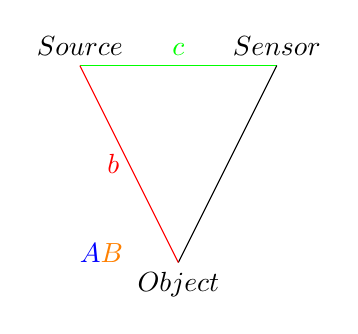
\begin{tikzpicture}[scale=2.5]

		\coordinate [label={[black]above:$Source$}] (A) at (0, 1);
		\coordinate [label={[black]above:$Sensor$}] (B) at (1, 1);
		\coordinate [label={[black]below:$Object$}] (C) at (0.5, 0);

		\draw[green] (A) -- node [above] {$c$} (B);
		\draw[black] (B) -- node [right] {$ $} (C);
		\draw[red] (C) -- node [left] {$b$} (A);

		\tkzMarkAngle[fill=white, size=0.25cm,%
		opacity=1](C,A,B)
		\tkzLabelAngle[pos=0.15](C,A,B){$\color{blue}A$}

		\tkzMarkAngle[fill=white,size=0.25cm,%
		opacity=1](A,B,C)
		\tkzLabelAngle[pos=-0.15](C,B,A){$\color{orange}B$}

		% \tkzMarkAngle[fill=green,size=0.25cm,%
		% opacity=.4](B,C,A)
		% \tkzLabelAngle[pos= 0.15](B,C,A){$ $}

		\end{tikzpicture}
	\end{subfigure}
	\caption{Triangulation 3D scanners \cite{Form2014}}
	\label{fig:triangulation-scanners}
\end{figure}

Triangulation scanners, as the name suggests, uses trigonometric triangulation \cite{Frohlich2004} to locate a point in a scene relative to scanner. Triangulation can be performed by either emitting a laser pulse, laser bear or by projecting a series of linear light patterns and then picking up the reflection with a sensor at a known position. During laser triangulation, the displacement of the object affects the angle at which the laser is returned (see \autoref{fig:triangulation-scanners}). Using structured light, the distortions in the patterns from the sensor's perspective can be used to determine the angle of reflected light \cite{Brown2012}. Given the precise distance between the light source and sensor ($\begingroup\color{green}c\endgroup$) and as well as the outgoing angle of emitted light ($\begingroup\color{blue}A\endgroup$) and incoming angle of reflected light ($\begingroup\color{orange}B\endgroup$), the distance to the object is given by $\begingroup\color{red}b\endgroup = \begingroup\color{green}c\endgroup\frac{ sin(\begingroup\color{orange}B\endgroup)}{sin(\pi - \begingroup\color{blue}A\endgroup-\begingroup\color{orange}B\endgroup)}$.

\subsection{Time of flight scanners (TOF)}

\begin{figure}[ht]
  \centering
  \includegraphics[width=.5\linewidth]{images/pulse-tof}
  \caption{Time of flight scanner}
  \label{fig:tof}
\end{figure}

Time of flight scanners emit laser pulses and measure the time it takes for a pulse reflection to be detected by the scanner's sensor (see \autoref{fig:tof}). Given the speed of light, the distance traveled by the light can be determined. Given the time it takes for light to travel to a surface and back to the scanner ($t$), the distance ($d$) is given by $d = ct/2$ where $c$ is the speed of light. The accuracy of the distance calculation depends on how precisely time can be measured \cite{Form2014}.

\begin{figure}[b]
	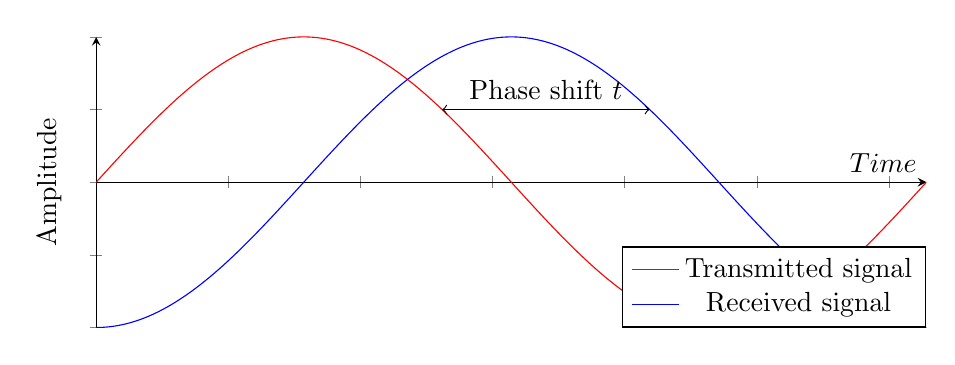
\begin{tikzpicture}[scale=1]
	\begin{axis}[
		width=1\textwidth,
		height=150,
	    axis lines = left,
	    yticklabels={,,},
	    xticklabels={,,},
	    axis x line=center,
	    xlabel = $Time$,
	    ylabel = {Amplitude},
	    legend style={
	    at={(1,0)},
	    anchor=south east}]
	]
	\addplot[samples=500,domain=0:2*pi, color=red]{sin(deg(x))};
	\addlegendentry{Transmitted signal}
	\addplot[samples=500,domain=0:2*pi, color=blue]{sin(deg(x-pi/2))};
	\addlegendentry{Received signal}
	\draw[<->] (axis cs:2.61799,0.5) -- node[above]{Phase shift $t$} (axis cs:4.18879,0.5);
	\end{axis}
	\end{tikzpicture}
	\caption{Phase shift in returned signal}
	\label{fig:phase-shift}
\end{figure}

Laser phase-shift scanners \cite{Frohlich2004} are a variation on the standard TOF scanner. These scanners modulate the power of the laser pulse in a sinusoidal wave during a scan. The phase shift in the returning pulse is used to compute the round trip time (see \autoref{fig:phase-shift}). Due to the cyclical nature of the signal, phase shift is ambiguous. This ambiguity is resolved by using measurements at multiple frequencies \cite{Bhurtha}.



\subsection{Comparison}

Triangulation scanners can achieve 10 micrometer accuracy over distances less than one meter. Over longer distances the triangle in \autoref{fig:triangulation-scanners} becomes to long and the distance calculation error prone. Structured light scanners tend to be faster than laser scanners as the whole scene is captured instead of a single point at a time \cite{Brown2012}. Scanners are also less prone to motion distortions. Hand held scanners of this type exists which reduces setup time compared to other scanners.

Time of flight scanners can measure a round trip of a laser pulse to an object more accurately over long distances than triangulation scanners can measure perspective distortions. This technology does not however deal well with distances less than 2 meters. Pure TOF scanners can scan distances up to 1000 meters \cite{Form2014}. TOF scanners can be set to sample at different resolutions. Low resolution scans (10 000 points) may take seconds while higher resolution scans (millions of points) may take minutes.

Phase-based scanners are more limited in range due to the ambiguity of returned signals from beyond the design distance \cite{Bhurtha}. Objects from beyond the scanner's designed range can sometimes be at closer distances when the scanner software fails to discard far away points. Phase based scanners make up for this shortfall by being much faster and more accurate within its range \cite{Form2014}.


\begin{table}
\begin{tabular}{ |l|l|l|l|l|l| }
  \hline
  Type &              Range &        Precision       & Speed & Portability \\
  \hline
  Structured light &    <1m     & 10 micrometer  & Seconds & High \\
  Laser triangulation & <1m     & 10 micrometer  & Seconds  & Medium \\     
  TOF &                 2-1000m & Medium      & Minutes & Low \\
  Phase &               2-100m & Low         & Seconds to Minutes & Low \\
  \hline  
\end{tabular}
\caption{Comparison of scanning technology}
\end{table}


\subsection{Data}

The terrestrial laser scanners described above all produce angle and range measurements that are converted into 3D coordinates relative to the scanner. Scanners also record the intensity of the light returned. High end scanners sometimes have integrated cameras that are used to map colors to captured data points \cite{Frohlich2004}. Orientation and GPS measurements are also available in some models which help speed up registration (\todo{see section X}).

Scanner manufacturers may also record lower level measurements that are specific to their scanners. This data may valuable in cleaning artifacts from scans. However, this data tends to be locked away in propriety formats which are not readily accessible. We therefore limit our investigation to data that can be readily exported from scanner software. We also do not consider color information as such datasets were not readily available for this work.

% (Mention non uniform point density somewhere? too obvious?)
% (Mention scanner resolution increasing over time?)

\subsection{Artifacts} \label{sec:artifacts}

In addition to the phase binning issues which occur in phase-based TOF scanners, scanners are subject to a number of other limitations. Due to the optical nature of the above scanners \todo{why did Patrick underline above scanners?}, difficulties are often encountered when dealing with shiny, mirroring or transparent objects. Windows cannot be captured as light passes through without being reflected. Mirror-like surfaces are also missed because light does not reflect back towards the scanner. The sun and other bright objects and cause points not associated with any physical object to appear in a scan. Fog and smoke can also cause problems.

\todo[inline]{More detail on artifacts}

\begin{figure}[ht]
  \centering
  \includegraphics[width=1\linewidth]{images/mixed-pixel}
  \caption{Mixed pixels. Green are valid points and red are not. \cite{Tuley2005}}
  \label{fig:mixed-pixel}
\end{figure}

Mixed pixels is another problematic aspect of laser scanning. When a laser pulse partially hits a near and then subsequently a far object, the result is a data point between the near and far object \cite{Tuley2005} (see \autoref{fig:mixed-pixel}).


Time of flight scanners are generally used in the cultural heritage domain because of their long range, these scanners will be the focus of our research.


\section{3D reconstruction pipeline} \label{sec:pipeline}


\begin{figure}

	% Define block styles
	\tikzstyle{decision} = [diamond, draw, fill=blue!20, 
	    text width=4.5em, text badly centered, node distance=3cm, inner sep=0pt]
	\tikzstyle{block} = [rectangle, draw, fill=gray!20, 
	    text width=5em, text centered, rounded corners, minimum height=4em]
	\tikzstyle{optionalblock} = [rectangle, draw, dashed,
	    text width=5em, text centered, rounded corners, minimum height=4em]
	\tikzstyle{line} = [draw, -latex']
	\tikzstyle{cloud} = [draw, ellipse,fill=red!20, node distance=3cm,
	    minimum height=2em]
	
	\centering

	\begin{tikzpicture}[node distance = 2cm, auto]
	    % Place nodes
	    \node [block] (acquire) {Scan acquisition};

	    \node [optionalblock, below right of=acquire, node distance=3cm] (clean) {\bf{Clean}};
	    \node [block, below left of=acquire, node distance=3cm] (register) {Register};
	    \node [block, below of=acquire, node distance=4cm] (reconstruct) {Reconstruct surface};
	    \node [optionalblock, right of=reconstruct, node distance=3cm] (autofill) {Automatic hole filling};
	    \node [optionalblock, left of=reconstruct, node distance=3cm] (filling) {Manual hole filling};
	    \node [block, below of=reconstruct, node distance=2cm] (texture) {Texture};
	    % Draw edges
	    \path [line] (acquire) -- (clean);
	    \path [line] (acquire) -- (register);
	    \path [line][<->] (clean) -- (register);
	    \path [line] (register) -- (reconstruct);
	    \path [line][-] (reconstruct) -- (autofill);
	    \path [line] (reconstruct) -- (filling);
	    \path [line] (filling) -- (texture);
	    \path [line] (reconstruct) -- (texture);
	    % \path [line] (decide) -| node [near start] {yes} (update);
	    % \path [line] (update) |- (identify);
	    % \path [line] (decide) -- node {no}(stop);
	    % \path [line,dashed] (expert) -- (acquire );
	    % \path [line,dashed] (system) -- (acquire );
	    % \path [line,dashed] (system) |- (evaluate);

	    \draw[densely dotted] (1.7,-5.3) rectangle (4.7,-6.7);

	    % legend
	    \node [block, right of=texture, node distance=2.5cm, scale=0.7,
	    	text width=3.8em, minimum height=1em](required) {Required step};
	    \node [optionalblock, right of=required, node distance=1.4cm, scale=0.7,
	    	text width=3.8em, minimum height=1em] (notrequired) {Optional step};

	\end{tikzpicture}

	\caption{Reconstruction pipeline.}
	\label{fig:pipeline}

\end{figure}


3D reconstruction of a site starts with the acquisition of range scans in the field. The collection of raw scans are then subject to a series of processing steps. Unwanted objects and noise may need to be removed and missing data could be synthesized. The scans then need to transformed to coincide on a common coordinate frame in a process called registration. A surface model can then be constructed from the registered point sets. The final model is complete when the reconstructed mesh is textured (see \autoref{fig:pipeline}).

\subsection{Data acquisition}
Some degree of planning is required to ensure a successful 3d reconstruction of a heritage site. One needs to decide on an appropriate level of scan detail for different areas as the set resolution of a scanner determines the data acquisition rate. Scanner positions that result in flat angles of incidence with surfaces should be avoided to maximize surface detail. Choosing good scanning positions will ensure that maximum site coverage is achieved in the most economical way \cite{Ruther2011}.

Some additional consideration can speed up later steps in the pipeline. Automated registration tools require requires that that overlap between scans are achieved. Positioning the scanner in the same level orientation also helps with registration \cite{Ruther2011}.

\subsection{Registration}  

\begin{figure}[ht]
  \centering
  \includegraphics[width=0.6\linewidth]{images/registration}
  \caption{ICP correspondences. (source PCL) }
  \label{fig:mixed-pixel}
\end{figure}

Two approaches exist to transform all scans onto a uniform coordinate system. The first approach requires placing reference objects, called targets, around a site during data acquisition. When the same object is found in two scans, the object's shape can be used to align the scans. The second approach is called Iterated Closest Point (ICP) that aligns scans by using surface features \cite{Besl1992}.

Automated software make targets are easy to identify and provides highly accurate registration. They do however have to captured in high resolution in order to be useful. This may require one to capture more scans than what is required for documentation purposes. In the heritage domain they have been found to be impractical as they often need to be placed in hard to reach places and intricate indoor environments require too many targets \cite{Ruther2011}. 

ICP requires less effort during data acquisition. The procedure however does not lend itself to as high a level of automated registration. The algorithm requires that two surfaces are roughly aligned as an initial condition. Correspondences are then computed between the surfaces where after an incremental transformation is computed to minimize the distance between all the correspondences. After the transformation is applied, the procedure is repeated until convergence is reached. There are many variations to the ICP algorithm that vary mainly on the type of correspondent matching and optimization procedure used \cite{Besl1992}.  

A user needs to ensure a good initial alignment or no convergence may be achieved. Featureless surfaces are also problematic as the optimization problem will have multiple solutions which may lead to misalignment.

\subsection{Cleaning}

\begin{figure}[ht]
	\begin{subfigure}[b]{.45\textwidth}
	  \centering
	  \includegraphics[width=.9\linewidth]{images/dirty}
	  % \caption{Structured light 3D scanning \cite{Form2014}}
	  % \label{fig:structured-light-scan}
	\end{subfigure}%
	\begin{subfigure}[b]{.45\textwidth}
	  \centering
	  \includegraphics[width=.9\linewidth]{images/clean}
	  % \caption{Laser 3D scanning}
	  % \label{fig:images/triangulate-laser-scan}
	\end{subfigure}
  \caption{Trees cleaned from a scan}
  \label{fig:cleaning}
\end{figure}

Cleaning is not an important step for documentation purposes but neglecting it in the modeling pipeline will lead to displeasing results. Trees, people, cables, cars, doors, animals and other random unwanted objects as well as scanner artefacts as mentioned in \autoref{sec:artifacts} are removed during the cleaning process. 




 be used if it available. Alternatively photos from the site has to be mapped to the model. The second approach is somewhat more time consuming.

is the process of aligning all the scans on a common coordinate system (mention Iterative closest points?)

The cleaning step can be omitted but the quality of the model will be affected. Objects such as trees or grass do not always mesh nicely, and floating bits of people as they walk around may not be aesthetically pleasing. Hole filling is also not strictly necessary. It can even be argued that it compromises the integrity of the historical record as the filled area would be fabricated.

The first 3 step also do not have to happen in order. It is often the case that hole filling, cleaning and registration tasks are interspersed. Cleaning may be detrimental to the reregistration process as useful correspondences may be removed. Cleaning scans after registration can however be problematic. If the scans have been merged into a single point cloud, loading the scan into main memory may not be an option on some programs. One also loses the 2d grid structure of the scan after merging. The scan's grid allows one to interpret the scan as a 2d image which may be easier to clean.





% \section{Point cloud cleaning} \label{sec:cleaning}
% 	Focused specifically on the task of point cloud cleaning in heritage scenes

% 	\subsection{Problem}
% 	Characterize heritage scenes
% 	\begin{itemize}
% 		\item Large scans
% 		\item many scans
% 		\item Non uniform density
% 		\item Large point sets
% 		\item Hard to distinguish trees from walls
% 	\end{itemize}

% 	\subsection{Existing systems}
% 		\begin{itemize}
% 			\item Z\&Y
% 			\item Cyclone
% 			\item Pointools
% 			\item Meshlab
% 			\item VR Mesh Studio
% 			\item Carlson Pointcloud
% 			\item 3D Reshaper
% 			\item Terrascan
% 		\end{itemize}

% 	\subsection{Evaluation of existing systems}
% 	We should look at existing systems in terms of a testing framework
% 	Evaluate their tools
% 	Evaluate user interface
% 	\begin{itemize}
% 		\item navigation: camera vs object move
% 		\item tool set (what tools are available)
% 		\item license
% 		\item 2d/3d editing
% 		\item extensibility (why did I not use it)
% 	\end{itemize}

		

% \section{Summary}
% %What do I conclude from all this and lead into the next chapter.	



% \section{Review of literature}

% \cite{Spina2010} Cultural heritage segmentation

